\documentclass[12pt]{article}

% Language setting
% Replace `english' with e.g. `spanish' to change the document language
\usepackage[english]{babel}

% Set page size and margins
% Replace `letterpaper' with`a4paper' for UK/EU standard size
\usepackage[letterpaper,top=2cm,bottom=2cm,left=3cm,right=3cm,marginparwidth=1.75cm]{geometry}

% Useful packages
\usepackage{amsmath}
\usepackage{graphicx}
\usepackage[colorlinks=true, allcolors=blue]{hyperref}
\usepackage{indentfirst}

\title{Project Proposal: Parallel Cellular Automata}
\author{Zacree Carroll, Troy Clendenen, Raul Patel}

\begin{document}
\maketitle

%\begin{abstract}
%Your abstract.
%\end{abstract}

\section{Introduction}
\subsection{What is Cellular Automata}
A cellular automaton is a single system with a collection of cells. The state of a cell during any particular discrete time step is governed by the combination of its previous state and the previous states of its neighbors. Complex behavior can arise from these systems (often governed by a simple set of rules). Figure 1 is an example of what is known as a "glider" in John Conway's Game of Life. Gliders are one of the more famous patterns in Game of Life. They emerge after a certain time step and they will move diagonally across the screen oscillating through the different forms shown in the example. This is but one of many entities which arise from the simple set of rules of which Game of Life is composed. 

\begin{figure}[h]
\centering
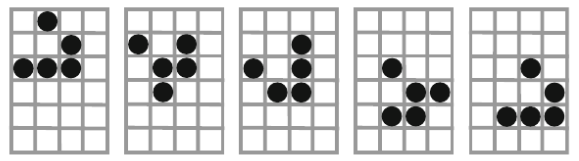
\includegraphics[width=0.5\textwidth]{5-stepGlider.PNG}
\caption{\label{fig:Glider}Five time steps of a glider.}
\end{figure}

\par 
\subsection{Interesting historical facts}
In the past computation of any particular cellular automata was considered impractical due to the modality of computing at that time and the nature of the differential equations which were used to describe them.\cite{Cann95} Recent breakthroughs in the field of parallel computation have provided a more practical framework within which cellular automata can be modelled. Cellular automata were first designed by John Von Neumann in the 1950s as a way to study self-replicating systems.\cite{neumann} Since their conception cellular automata have primarily been used to study parallel computing methodology but have also been used to simulate a wide variety of phenomena.\cite{Cann95} 

\par
\section{Different Problems in Cellular Automata}
\subsection{Simulation of Wild Fires}
Cellular automata are frequently used in computational simulation. One such area that is quite popular is the simulation of wild fires. Many of the approaches to this problem vary in their considerations for their  particular model but the majority of them share the goal of predicting wild fire behavior given a set of input parameters. Some of those input parameters may include cell size, moisture levels, weather patterns, and the heterogeneity of the area. Different collections of these parameters are referred to as fire models and one such fire model is the EMBYR model. 

\begin{figure}[h]
\centering
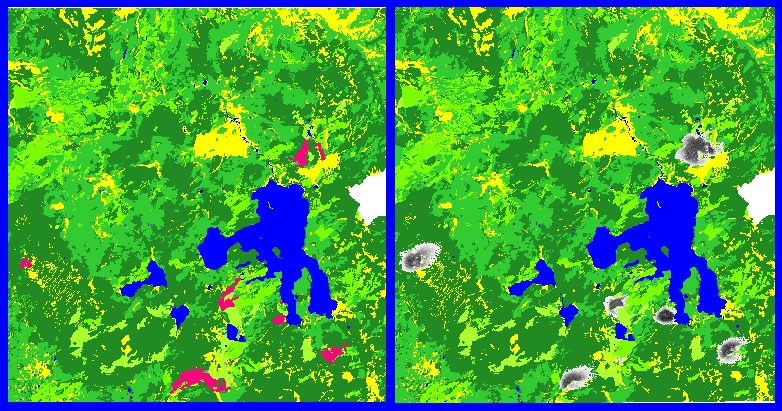
\includegraphics[width=0.5\textwidth]{embyr.PNG}
\caption{\label{fig:Fire}Example image of an EMBYR simulation.}
\end{figure}

\par
The EMBYR model has a cell size of 50m. The considerations that this model makes are diffusive spread from cell to cell, the effects of windspeed and direction, distant cell ignition due to firebrands (an object which is airborne and carried some distance in an airstream), and differing combustibility throughout the landscape due to variance in moisture.\cite{HARGROVE2000243}

\subsection{Simulation of Bioremediation}
Another use of the cellular automata approach can be found in the simulation of bioremedation. Bioremediation involves contaminated soils and the use of organisms such as bacteria as a means of site clean-up. Previously before massively parallel computing was available this problem was only capable of being modelled by differential calculus and the use of such a method had to negate some of the nuance of the interactions taking place. By using the cellular automata approach such negations become unnecessary.\cite{Gregorio96aparallel}

\par
\section{Possible Directions for the Project}
\subsection{Implementing a Parallel CA Simulation}
Parallelizing cellular automata is not a  new idea. On the other hand, it's almost inherent given the amount of local interactions cells may have with each other, and essential in order to implement large-scale simulations. There have been many projects that have designed and implemented parallel models of CA, such as CAMEL, StarLogo, NEMO, and CAPE \cite{Talia2007CellularA}. While our group does not expect to create a system as sophisticated as any of these, our main direction is to simply design and implement one such parallel cellular automata application using OpenMP. Ideally, we'd like to parallelize a forest fire simulation using CA. However, depending on our ability to deal with a complex idea for a simulation, we may deliver a project with a simpler set of rules (such as Conway's Game of Life \cite{Adamatzky2010GameOL}).

\par
\subsection{Optimizing Simulations for Shared-Memory Systems}
Utilizing the benefits of specific architectures is important in parallel computing, along with HPC as a whole. Data locality is one of the most important concepts in optimizing high-performance codes in computer science. One such concept that exists to help take advantage of locality is Partitioned Global Address Space (PGAS). While we don't think anyone in our group can implement an incredibly sophisticated system, it might be nice to try and implement a way for our specific application to take advantage of manycore CPU clusters using MPI. MPI has actually been shown to be a decent alternative to a native implementation for PGAS functionality in situations when one may not be readily available \cite{Daily2014OnTS}. While there may be better approaches to this, given the scope of the class and the concepts we will be learning, it might be a good idea to work on this if we have time in order to gain more experience with MPI.

\begin{figure}[h]
\centering
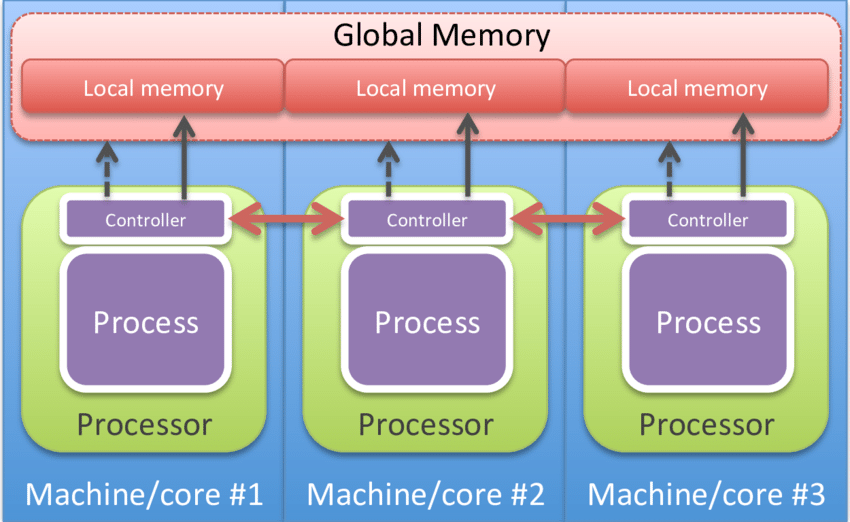
\includegraphics[width=0.5\textwidth]{pgas.png}
\caption{\label{fig:PGAS}Basic outline of a PGAS runtime.}
\end{figure}

\par
\subsection{Analyzing Parallelizable Code Segments}
While it may not contribute to explicit parallel programming experience, writing static analysis tools to assist our group to develop and improve our project is something that might be helpful to work on. It would also help us understand how compilers analyze and work with parallel programs. Most analysis would probably involve loops and memory access patterns, and we could use things like the polyhedral model to potentially transform and optimize our loop structure. While it's unlikely our group goes down this path, it's something that's interesting to think about going in the future.

\par
\section{Expected Results}
\subsection{Base Project Deliverables}
As stated earlier, we are intending to start with our own implementation of a parallel CA simulation. By doing so, we hope we can better determine how to expand upon the basic structure of CA. Because of this, we know at the very least we want to build our own Conway's Game of Life simulation using C++ and OpenMP. Because many cell-to-cell interactions are inherently parallel within CA simulations (and there is no real reason to write serial CA applications), we want to evaluate our project with weak scaling in mind. There's merit in comparing serial vs parallel execution time, however our group's focus will be on the scalability of our model. We plan on increasing the number of cells for each simulation to scale the problem size and evaluate our program's performance for each size on a single node. Hopefully our project can scale relatively well given time constraints of the term, and if we have time, there are a few more things we'd like to be able to include in our final submission.

\par
\subsection{Expanding the Project if Time Allows}
\subsubsection{Streamlined API For Generalizing Parallel CA Simulations}
One thing that would be really great to work on is a more generalized API that can be used in designing parallel CA simulations. While the Game of Life is cool, creating an API to help other scientists design their own simulations is something that really interests us. We'd keep our focus on streamlined parallelization of these applications, and attempt to keep the same level of efficiency that we hope to achieve with our base project. This could also support extensions of CA simulations to non-academic areas, such as assigning musical notes to different stages of the cells to use as a software instrument. There have been other projects made for the purpose of general scientific simulations using CA, however our idea is that this would give us experience with parallel computing in context of general software engineering practices.

\par
\subsubsection{Further Optimizations}
We'd like to utilize the machines to the best of our abilities in this project, and if all goes well with our initial build, then we'd like to also design a PGAS runtime using MPI to improve our application's scalablity by utilizing multiple CPU nodes efficiently. If our group manages to design a working PGAS runtime for this project, then we would make sure to compare program performance with multiple CPU nodes to performance without utilizing multiple CPU nodes. We could even test strong vs weak scaling in the context of our project and see how well it line up with Ahmdal's law and Gustafson's law. Hopefully this could provide us with further insight in the nature of CA problems, however this may be unlikely within the scope of this class.

%\subsection{How to create Sections and Subsections}

%Simply use the section and subsection commands, as in this example document! With Overleaf, all the formatting and numbering is handled automatically according to the template you've chosen. If you're using Rich Text mode, you can also create new section and subsections via the buttons in the editor toolbar.

%\subsection{How to include Figures}

%First you have to upload the image file from your computer using the upload link in the file-tree menu. Then use the includegraphics command to include it in your document. Use the figure environment and the caption command to add a number and a caption to your figure. See the code for Figure \ref{fig:frog} in this section for an example.

%Note that your figure will automatically be placed in the most appropriate place for it, given the surrounding text and taking into account other figures or tables that may be close by. You can find out more about adding images to your documents in this help article on \href{https://www.overleaf.com/learn/how-to/Including_images_on_Overleaf}{including images on Overleaf}.

%\begin{figure}
%\centering
%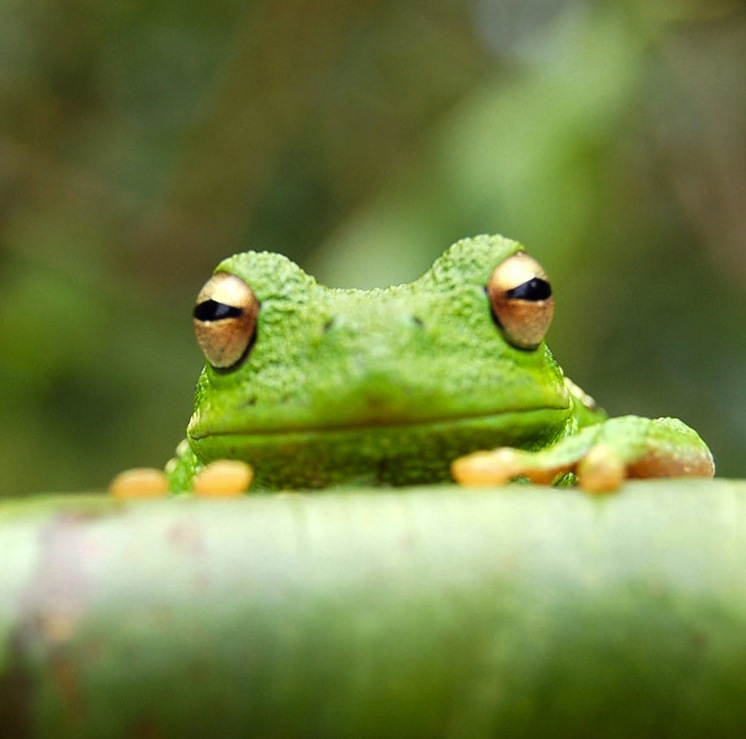
\includegraphics[width=0.3\textwidth]{frog.jpg}
%\caption{\label{fig:frog}This frog was uploaded via the file-tree menu.}
%\end{figure}

%\subsection{How to add Tables}

%Use the table and tabular environments for basic tables --- see Table~\ref{tab:widgets}, for example. For more information, please see this help article on \href{https://www.overleaf.com/learn/latex/tables}{tables}. 

%\begin{table}
%\centering
%\begin{tabular}{l|r}
%Item & Quantity \\\hline
%Widgets & 42 \\
%Gadgets & 13
%\end{tabular}
%\caption{\label{tab:widgets}An example table.}
%\end{table}

%\subsection{How to add Comments and Track Changes}

%Comments can be added to your project by highlighting some text and clicking ``Add comment'' in the top right of the editor pane. To view existing comments, click on the Review menu in the toolbar above. To reply to a comment, click on the Reply button in the lower right corner of the comment. You can close the Review pane by clicking its name on the toolbar when you're done reviewing for the time being.

%Track changes are available on all our \href{https://www.overleaf.com/user/subscription/plans}{premium plans}, and can be toggled on or off using the option at the top of the Review pane. Track changes allow you to keep track of every change made to the document, along with the person making the change. 

%\subsection{How to add Lists}

%You can make lists with automatic numbering \dots

%\begin{enumerate}
%\item Like this,
%\item and like this.
%\end{enumerate}
%\dots or bullet points \dots
%\begin{itemize}
%\item Like this,
%\item and like this.
%\end{itemize}

%\subsection{How to write Mathematics}

%\LaTeX{} is great at typesetting mathematics. Let $X_1, X_2, \ldots, X_n$ be a sequence of independent and identically distributed random variables with $\text{E}[X_i] = \mu$ and $\text{Var}[X_i] = \sigma^2 < \infty$, and let
%\[S_n = \frac{X_1 + X_2 + \cdots + X_n}{n}
 %     = \frac{1}{n}\sum_{i}^{n} X_i\]
%denote their mean. Then as $n$ approaches infinity, the random variables $\sqrt{n}(S_n - \mu)$ converge in distribution to a normal $\mathcal{N}(0, \sigma^2)$.


%\subsection{How to change the margins and paper size}

%Usually the template you're using will have the page margins and paper size set correctly for that use-case. For example, if you're using a journal article template provided by the journal publisher, that template will be formatted according to their requirements. In these cases, it's best not to alter the margins directly.

%If however you're using a more general template, such as this one, and would like to alter the margins, a common way to do so is via the geometry package. You can find the geometry package loaded in the preamble at the top of this example file, and if you'd like to learn more about how to adjust the settings, please visit this help article on \href{https://www.overleaf.com/learn/latex/page_size_and_margins}{page size and margins}.

%\subsection{How to change the document language and spell check settings}

%Overleaf supports many different languages, including multiple different languages within one document. 

%To configure the document language, simply edit the option provided to the babel package in the preamble at the top of this example project. To learn more about the different options, please visit this help article on \href{https://www.overleaf.com/learn/latex/International_language_support}{international language support}.

%To change the spell check language, simply open the Overleaf menu at the top left of the editor window, scroll down to the spell check setting, and adjust accordingly.

%\subsection{How to add Citations and a References List}

%You can simply upload a \verb|.bib| file containing your BibTeX entries, created with a tool such as JabRef. You can then cite entries from it, like this: . Just remember to specify a bibliography style, as well as the filename of the \verb|.bib|. You can find a \href{https://www.overleaf.com/help/97-how-to-include-a-bibliography-using-bibtex}{video tutorial here} to learn more about BibTeX.

%If you have an \href{https://www.overleaf.com/user/subscription/plans}{upgraded account}, you can also import your Mendeley or Zotero library directly as a \verb|.bib| file, via the upload menu in the file-tree.

%\subsection{Good luck!}

%We hope you find Overleaf useful, and do take a look at our \href{https://www.overleaf.com/learn}{help library} for more tutorials and user guides! Please also let us know if you have any feedback using the Contact Us link at the bottom of the Overleaf menu --- or use the contact form at \url{https://www.overleaf.com/contact}.

\bibliographystyle{alpha}
\bibliography{bibCol}

\end{document}